
\documentclass[12pt]{exam}
\usepackage{amsthm}
\usepackage{libertine}
%\usepackage[utf8]{inputenc}
\usepackage[margin=1in]{geometry}
\usepackage{amsmath,amssymb}
\usepackage{multicol}
\usepackage[shortlabels]{enumitem}
\usepackage{siunitx}
\usepackage{cancel}
\usepackage{graphicx}
\graphicspath{{./}}
\usepackage{pgfplots}
\usepackage{hyperref}
\usepackage{listings}
\usepackage{tikz}
\usepackage{minted}
\def\code#1{\texttt{#1}}
\usepackage{amssymb}
\usepackage{xcolor}
% for plotting
\usepackage{pgfplots}
\pgfplotsset{compat=1.16}
\usepackage{tikz}
\usetikzlibrary{arrows.meta}

\newcommand{\quotebox}[1]
{
  \begin{center}
    \fcolorbox{white}{blue!15!gray!15}{
      \begin{minipage}{0.7\linewidth}\vspace{10pt}
        \center
        \begin{minipage}{0.8\linewidth}{\space\Huge``}{\setlength{\parindent}{1.5em}#1}{\hspace{1.5em}\break\null\Huge\hfill''}
        \end{minipage}
        \smallbreak
      \end{minipage}
    }
\end{center}
}

%\DeclareUnicodeCharacter{2212}{-}


\let\oldemptyset\emptyset
\let\emptyset\varnothing

\hypersetup{
    colorlinks=true,
    linkcolor=blue,
    filecolor=magenta,      
    urlcolor=cyan,
    pdftitle={Overleaf Example},
    pdfpagemode=FullScreen,
    }
    
\urlstyle{same}

\pgfplotsset{width=10cm,compat=1.9}
\usepgfplotslibrary{external}
\tikzexternalize

\newcommand{\class}{Math 415} % This is the name of the course 
\newcommand{\examnum}{Homework-1} % This is the name of the assignment
\newcommand{\examdate}{September 14} % This is the due date
\newcommand{\timelimit}{}

\newcommand{\BO}{\mathcal{O}}




\begin{document}
\pagestyle{plain}
\thispagestyle{empty}

\noindent
\begin{tabular*}{\textwidth}{l @{\extracolsep{\fill}} r @{\extracolsep{6pt}} l}
\textbf{\class} & \textbf{Name:} & \textit{Zhenzhao Tu}\\ %Your name here instead, obviously 
\textbf{\examnum} &&\\
\textbf{\examdate} &&\\
\end{tabular*}\\
\rule[2ex]{\textwidth}{2pt}
% --

\section{Problem 1}
\begin{enumerate}[(a)]
    \item To write the second-order ordinary differential equation 
	  \[x'' + \mu(1-x^2)x' + x = 0\]
	in a system of first-order ordinary differential equations, you can introduce new variables to break it down. Let's set:
	\[x_1 = x ,\quad x_2 = x'\]
	Now we can write two first-order equations using these new variables:
	\[x'_1 = x_2 ,\quad x'_2 = \mu (1-x_1^2)x_2 - x_1\]
	So the system of equations in the form \(x'_i = f_i(x_1, x_2)\) would be:
	\[\begin{cases}
		x'_1 = x_2 \\
		x'_2 = \mu (1-x_1^2)x_2 - x_1
	\end{cases}\]
	
     \item To write the third-order ordinary differential equation
	  \[y''' + yy'' = 0\]
	in a system of first-order ordinary differential equations, you can introduce new variables to break it down. Let's set:
	\[y_1 = y ,\quad y_2 = y' ,\quad y_3 = y''\]
	Now we can write three first-order equations using these new variables:
	\[y'_1 = y_2 ,\quad y'_2 = y_3 ,\quad y'_3 = -y_1y_3\]
	So the system of equations in the form \(y'_i = f_i(y_1, y_2, y_3)\) would be:
	\[\begin{cases}
		y'_1 = y_2 \\
		y'_2 = y_3 \\
		y'_3 = -y_1y_3
	\end{cases}\]

     \item To write the second-order ordinary differential equation
	  \[x'' + \mu x' = \cos t \]
	in a system of first-order ordinary differential equations, you can introduce new variables to break it down. Let's set:
	\[x_1 = x ,\quad x_2 = x'\]
	Now we can write two first-order equations using these new variables:
	\[x'_1 = x_2 ,\quad x'_2 = \cos t - \mu x_2\]
	So the system of equations in the form \(x'_i = f_i(x_1, x_2)\) would be:
	\[\begin{cases}
		x'_1 = x_2 \\
		x'_2 = \cos t - \mu x_2
	\end{cases}\]
	
     \item To write the second-order ordinary differential equation
	  \[\begin{cases}
		  x'' + y^2 = 0 \\
		  y'' - x^2 = 0
	  \end{cases}\]
	in a system of first-order ordinary differential equations, you can introduce new variables to break it down. Let's set:
	\[x_1 = x ,\quad x_2 = x' ,\quad y_1 = y ,\quad y_2 = y'\]
	Now we can write four first-order equations using these new variables:
	\[x'_1 = x_2 ,\quad x'_2 = -y_1^2 ,\quad y'_1 = y_2 ,\quad y'_2 = x_1^2\]
	So the system of equations in the form \(x'_i = f_i(x_1, x_2)\) would be:
	\[\begin{cases}
		x'_1 = x_2 \\
		x'_2 = -y_1^2 \\
		y'_1 = y_2 \\
		y'_2 = x_1^2
	\end{cases}\]
\end{enumerate}

\newpage
\section{Problem 2}
\begin{enumerate}[(a)]
	\item The graph of ODE \(x' = 5x^2 - 20\) is shown below:

		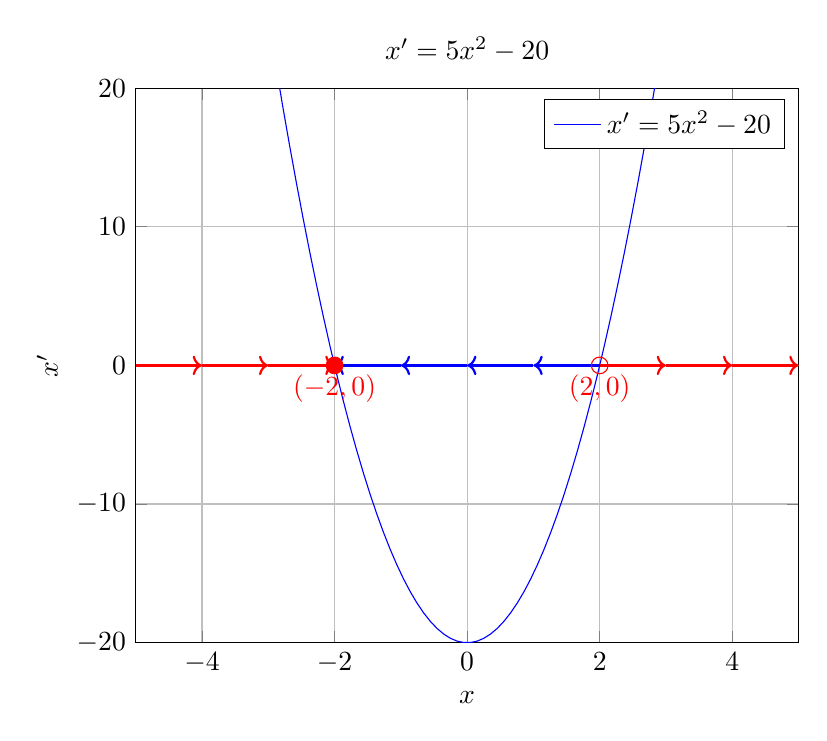
\begin{tikzpicture}
			% \draw[->,line width=2pt] (0,0) to (10,0);
		\begin{axis}[
			title={\(x' = 5x^2 - 20\)},
			xlabel={\(x\)},
			ylabel={\(x'\)},
			xmin=-5, xmax=5,
			ymin=-20, ymax=20,
			grid=both,
			]
		\addplot[blue, domain=-5:5, samples=100]{5*x^2 - 20};
		\addplot[orange, domain=-5:5, samples=100]{0};
		% add a red point at (2,0) and add lebal to the red point
		\addplot[only marks, mark=o, mark size=3pt, color=red] coordinates {(2,0)} node[anchor=north] {\((2,0)\)};
		% add a hollow point at (-2,0) and add lebal to the red point
		\addplot[only marks, mark=*, mark size=3pt, color=red] coordinates {(-2,0)} node[anchor=north] {\((-2,0)\)};

		% draw vector at (0, 0) toword (-1,0) and change the size of the arrow
		\addplot[->, thick, color=blue] coordinates {(0,0) (-1,0)};
		% vector from (-1,0) to (-2,0)
		\addplot[->, thick, color=blue] coordinates {(-1,0) (-2,0)};
		% vector from (1,0) to (0,0)	
		\addplot[->, thick, color=blue] coordinates {(1,0) (0,0)};
		% vector from (2,0) to (1,0)
		\addplot[->, thick, color=blue] coordinates {(2,0) (1,0)};

		% vector from (-5,0) to (-4,0)
		\addplot[->, thick, color=red] coordinates {(-5,0) (-4,0)};
		% vector from (-4,0) to (-3,0)
		\addplot[->, thick, color=red] coordinates {(-4,0) (-3,0)};
		% vector from (-3,0) to (-2,0)
		\addplot[->, thick, color=red] coordinates {(-3,0) (-2,0)};

		% vector from (2,0) to (3,0)
		\addplot[->, thick, color=red] coordinates {(2,0) (3,0)};
		% vector from (3,0) to (4,0)
		\addplot[->, thick, color=red] coordinates {(3,0) (4,0)};
		% vector from (4,0) to (5,0)
		\addplot[->, thick, color=red] coordinates {(4,0) (5,0)};
		\legend{\(x' = 5x^2 - 20\)}
		\end{axis}
		\end{tikzpicture}
	
	\item The graph of ODE \(x' = e^{-x}\sin x\) is shown below:

		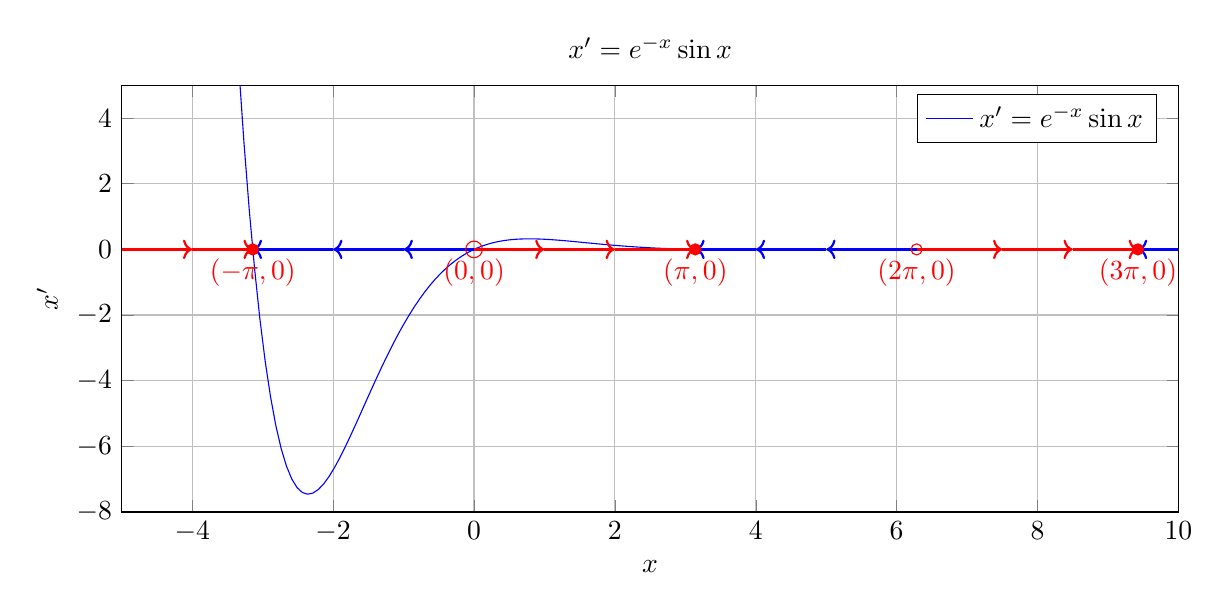
\begin{tikzpicture}
			% \draw[->,line width=2pt] (0,0) to (10,0);
		% edit width and height in option to change the size of the graph
		\begin{axis}[
			title={\(x' = e^{-x}\sin x\)},
			xlabel={\(x\)},
			ylabel={\(x'\)},
			xmin=-5, xmax=10,
			ymin=-8, ymax=5,
			grid=major,
			width=15cm,
			height=7cm,
			]
		\addplot[blue, domain=-5:10, samples=200]{e^(-x)*sin(deg(x))};
		\addplot[orange, domain=-5:10, samples=100]{0};

		% add a hollow red point at (0,0) and add lebal to the red point
		\addplot[only marks, mark=o, mark size=3pt, color=red] coordinates {(0,0)} node[anchor=north] {\((0,0)\)};
		% add a point at (\pi,0) and add lebal to the red point
		\addplot[only marks, mark=*, mark size=2pt, color=red] coordinates {(3.1415926,0)} node[anchor=north] {\((\pi,0)\)};
		% add a hollow point at (2\pi,0) and add lebal to the red point
		\addplot[only marks, mark=o, mark size=2pt, color=red] coordinates {(6.2831853,0)} node[anchor=north] {\((2\pi,0)\)};
		% add a point at (3\pi,0) and add lebal to the red point
		\addplot[only marks, mark=*, mark size=2pt, color=red] coordinates {(9.4247779,0)} node[anchor=north] {\((3\pi,0)\)};
		% add a point at (-\pi,0) and add lebal to the red point
		\addplot[only marks, mark=*, mark size=2pt, color=red] coordinates {(-3.1415926,0)} node[anchor=north] {\((-\pi,0)\)};

		% draw vector at (-5, 0) toword (-4,0) and change the size of the arrow
		\addplot[->, thick, color=red] coordinates {(-5,0) (-4,0)};
		% vector from (-4,0) to (-\pi,0)
		\addplot[->, thick, color=red] coordinates {(-4,0) (-3.1415926,0)};
		% vector from (-2,0) to (-\pi,0)
		\addplot[->, thick, color=blue] coordinates {(-2,0) (-3.1415926,0)};
		% vector from (-1,0) to (-2,0)
		\addplot[->, thick, color=blue] coordinates {(-1,0) (-2,0)};
		% vector from (0,0) to (-1,0)
		\addplot[->, thick, color=blue] coordinates {(0,0) (-1,0)};
		% vector from (0,0) to (1,0)
		\addplot[->, thick, color=red] coordinates {(0,0) (1,0)};
		% vector from (1,0) to (2,0)
		\addplot[->, thick, color=red] coordinates {(1,0) (2,0)};
		% vector from (2,0) to (\pi,0)
		\addplot[->, thick, color=red] coordinates {(2,0) (3.1415926,0)};
		% vector from (4,0) to (\pi,0)
		\addplot[->, thick, color=blue] coordinates {(4,0) (3.1415926,0)};
		% vector from (5,0) to (4,0)
		\addplot[->, thick, color=blue] coordinates {(5,0) (4,0)};
		% vector from (2\pi,0) to (5,0)
		\addplot[->, thick, color=blue] coordinates {(6.2831853,0) (5,0)};
		% vector from (2\pi,0) to (7.5,0)
		\addplot[->, thick, color=red] coordinates {(6.2831853,0) (7.5,0)};
		% vector from (7.5,0) to (8.5,0)
		\addplot[->, thick, color=red] coordinates {(7.5,0) (8.5,0)};
		% vector from (8.5,0) to (3\pi,0)
		\addplot[->, thick, color=red] coordinates {(8.5,0) (9.4247779,0)};
		% vector from (10,0) to (3\pi,0)
		\addplot[->, thick, color=blue] coordinates {(10,0) (9.4247779,0)};
		\legend{\(x' = e^{-x}\sin x\)}
		\end{axis}
		\end{tikzpicture}
	      
	      By analyzing the graph, we can see that the solution is periodic. The period is \(2\pi\).
	      Set \(x' = 0\), we can try to find the equilibrium points. Since \(e^{-x}\) will never be \(0\), we can set \(\sin x = 0\). So the equilibrium points are \(x = k\pi\), where \(k\) is an integer.
		
	\item The graph of ODE \(x' = 1 - 2 \cos x\) is shown below:

		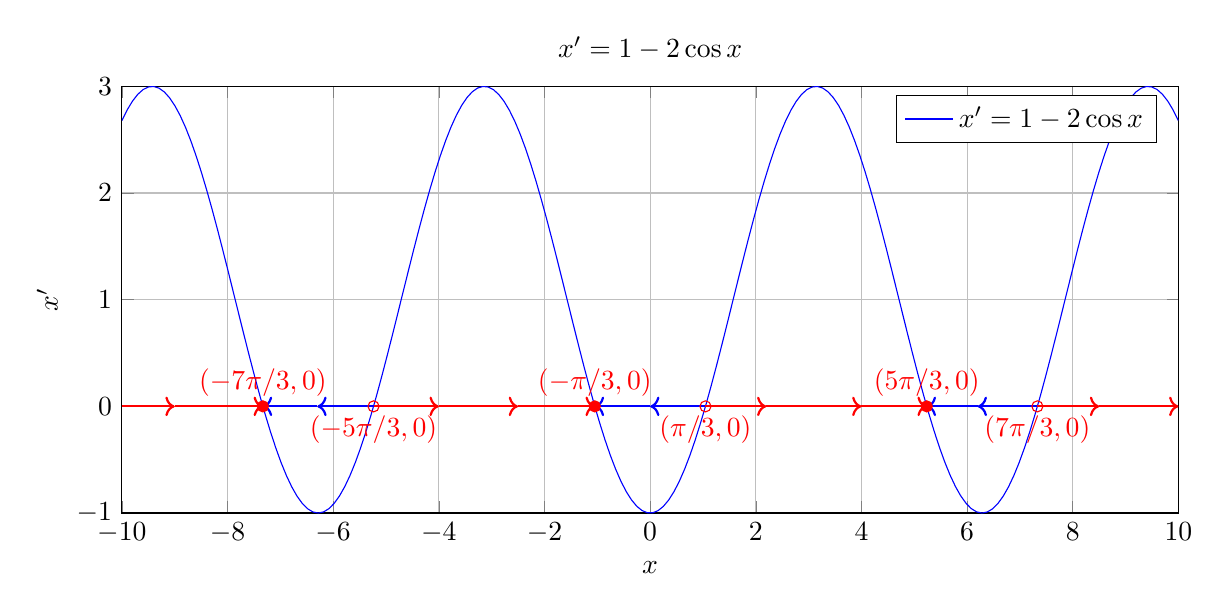
\begin{tikzpicture}
			% \draw[->,line width=2pt] (0,0) to (10,0);
		% edit width and height in option to change the size of the graph
		\begin{axis}[
			title={\(x' = 1 - 2 \cos x\)},
			xlabel={\(x\)},
			ylabel={\(x'\)},
			xmin=-10, xmax=10,
			ymin=-1, ymax=3,
			grid=major,
			width=15cm,
			height=7cm,
			]
		\addplot[blue, domain=-10:10, samples=200]{1-2*cos(deg(x))};
		\addplot[orange, domain=-10:10, samples=100]{0};

		% add a hollow red point at (\pi/3,0) and add lebal to the red point
		\addplot[only marks, mark=o, mark size=2pt, color=red] coordinates {(1.0471976,0)} node[anchor=north] {\((\pi/3,0)\)};
		% add a hollow point at (7\pi/3,0) and add lebal to the red point
		\addplot[only marks, mark=o, mark size=2pt, color=red] coordinates {(7.3303829,0)} node[anchor=north] {\((7\pi/3,0)\)};
		% add a hollow point at (-5\pi/3,0) and add lebal to the red point
		\addplot[only marks, mark=o, mark size=2pt, color=red] coordinates {(-5.2359878,0)} node[anchor=north] {\((-5\pi/3,0)\)};
		% add a point at (-\pi/3,0) and add lebal to the red point
		\addplot[only marks, mark=*, mark size=2pt, color=red] coordinates {(-1.0471976,0)} node[anchor=south] {\((-\pi/3,0)\)};
		% add a point at (-7\pi/3,0) and add lebal to the red point
		\addplot[only marks, mark=*, mark size=2pt, color=red] coordinates {(-7.3303829,0)} node[anchor=south] {\((-7\pi/3,0)\)};
		% add a point at (5\pi/3,0) and add lebal to the red point
		\addplot[only marks, mark=*, mark size=2pt, color=red] coordinates {(5.2359878,0)} node[anchor=south] {\((5\pi/3,0)\)};
		
		% draw vector at (-10, 0) toword (-9,0) and change the size of the arrow
		\addplot[->, thick, color=red] coordinates {(-10,0) (-9,0)};
		% vector from (-9,0) to (-7\pi/3,0)
		\addplot[->, thick, color=red] coordinates {(-9,0) (-7.3303829,0)};
		% vector from (-5\pi/3,0) to (-4,0)
		\addplot[->, thick, color=red] coordinates {(-5.2359878,0) (-4,0)};
		% vector from (-4,0) to (-2.5,0)
		\addplot[->, thick, color=red] coordinates {(-4,0) (-2.5,0)};
		% vector from (-2.5,0) to (-\pi/3,0)
		\addplot[->, thick, color=red] coordinates {(-2.5,0) (-1.0471976,0)};
		% vector from (\pi/3,0) to (2.2,0)
		\addplot[->, thick, color=red] coordinates {(1.0471976,0) (2.2,0)};
		% vector from (2.2,0) to (4,0)
		\addplot[->, thick, color=red] coordinates {(2.2,0) (4,0)};
		% vector from (4,0) to (5\pi/3,0)
		\addplot[->, thick, color=red] coordinates {(4,0) (5.2359878,0)};
		% vector from (7\pi/3,0) to (8.5,0)
		\addplot[->, thick, color=red] coordinates {(7.3303829,0) (8.5,0)};
		% vector from (8.5,0) to (10,0)
		\addplot[->, thick, color=red] coordinates {(8.5,0) (10,0)};

		% vector from (-6.3,0) to (-7\pi/3,0)
		\addplot[->, thick, color=blue] coordinates {(-6.3,0) (-7.3303829,0)};
		% vector from (-5\pi/3,0) to (-6.3,0)
		\addplot[->, thick, color=blue] coordinates {(-5.2359878,0) (-6.3,0)};
		% vector from (0,0) to (-\pi/3,0)
		\addplot[->, thick, color=blue] coordinates {(0,0) (-1.0471976,0)};
		% vector from (\pi/3,0) to (0,0)
		\addplot[->, thick, color=blue] coordinates {(1.0471976,0) (0,0)};
		% vector from (6.2, 0) to (5\pi/3,0)
		\addplot[->, thick, color=blue] coordinates {(6.2,0) (5.2359878,0)};
		% vector from (7\pi/3,0) to (6.2,0)
		\addplot[->, thick, color=blue] coordinates {(7.3303829,0) (6.2,0)};


		\legend{\(x' = 1 - 2 \cos x\)}
		\end{axis}
		\end{tikzpicture}

		By analyzing the graph, we can see that the solution is periodic. The period is \(2\pi\). When set \(x' = 0\), we can find the equilibrium points. Since \(\cos x\) equal to \(1/2\) when \(x = \pi/3 + 2k\pi\) or \(x = 5\pi/3 + 2k\pi\), where \(k\) is an integer. So the equilibrium points are \(x = \pi/3 + 2k\pi\) or \(x = 5\pi/3 + 2k\pi\), where \(k\) is an integer.

	\item The graph of ODE \(x' = e^x - \cos x\) is shown below:

		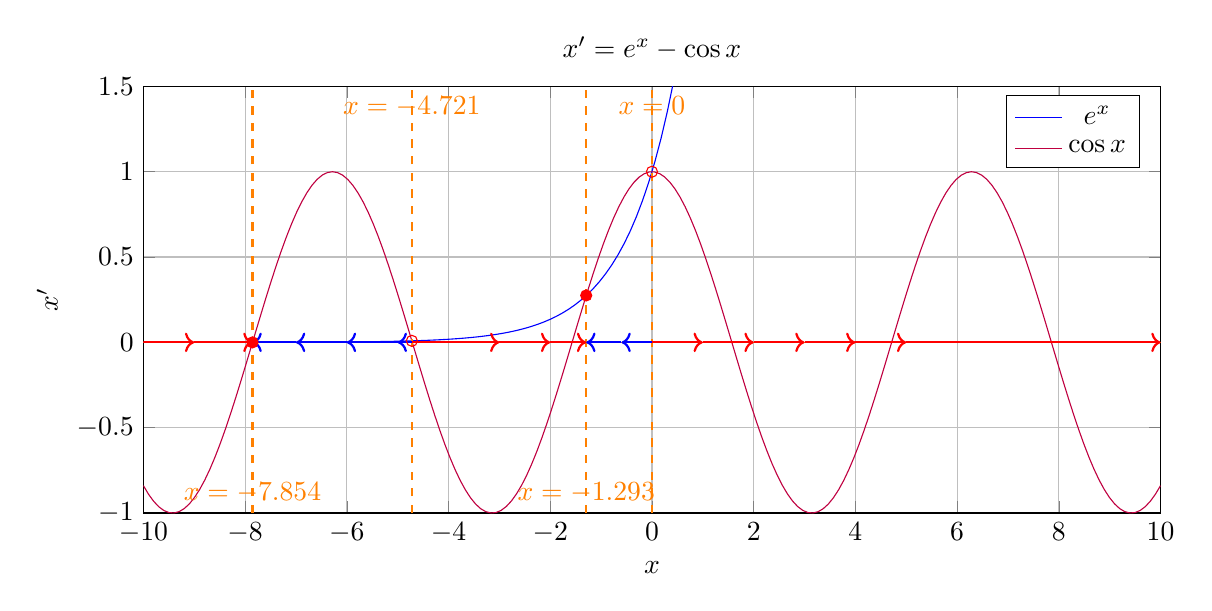
\begin{tikzpicture}
			% \draw[->,line width=2pt] (0,0) to (10,0);
		% edit width and height in option to change the size of the graph
		\begin{axis}[
			title={\(x' = e^x - \cos x\)},
			xlabel={\(x\)},
			ylabel={\(x'\)},
			xmin=-10, xmax=10,
			ymin=-1, ymax=1.5,
			grid=major,
			width=14.5cm,
			height=7cm,
			]
		\addplot[blue, domain=-10:2, samples=100]{e^x};
		\addplot[purple, domain=-10:10, samples=200]{cos(deg(x))};
		\addplot[orange, domain=-10:10, samples=100]{0};
		
		% add a hollow red point at (0,1) and add lebal to the red point
		\addplot[only marks, mark=o, mark size=2pt, color=red] coordinates {(0,1)};
		% add a point at (-1.293,0.275) and add lebal to the red point
		\addplot[only marks, mark=*, mark size=2pt, color=red] coordinates {(-1.293,0.275)};
		% add a hollow point at (-4.721,0.009) and add lebal to the red point
		\addplot[only marks, mark=o, mark size=2pt, color=red] coordinates {(-4.721,0.009)};
		% add a point at (-7.854,0) and add lebal to the red point
		\addplot[only marks, mark=*, mark size=2pt, color=red] coordinates {(-7.854,0)};

		% add a vertical dash line at x = 0 in orange color and add label to the line
		\addplot[orange, dashed, thick] coordinates {(0,-1) (0,1.5)} node[anchor=north] {\(x = 0\)};
		% add a vertical dash line at x = -1.293 in orange color and add label to the line
		\addplot[orange, dashed, thick] coordinates {(-1.293,-1) (-1.293,1.5)} node[pos=0, anchor=south] {\(x = -1.293\)};
		% add a vertical dash line at x = -4.721 in orange color and add label to the line
		\addplot[orange, dashed, thick] coordinates {(-4.721,-1) (-4.721,1.5)} node[anchor=north] {\(x = -4.721\)};
		% add a vertical dash line at x = -7.854 in orange color and add label to the line
		\addplot[orange, dashed, thick] coordinates {(-7.854,-1) (-7.854,1.5)} node[pos=0, anchor=south] {\(x = -7.854\)};
		
		% draw vector at (-10, 0) toword (-9,0) and change the size of the arrow
		\addplot[->, thick, color=red] coordinates {(-10,0) (-9,0)};
		% vector from (-9,0) to (-7.854,0)
		\addplot[->, thick, color=red] coordinates {(-9,0) (-7.854,0)};
		% vector from (-4.721,0) to (-3,0)
		\addplot[->, thick, color=red] coordinates {(-4.721,0) (-3,0)};
		% vector from (-3,0) to (-2,0)
		\addplot[->, thick, color=red] coordinates {(-3,0) (-2,0)};
		% vector from (-2,0) to (-1.293,0)
		\addplot[->, thick, color=red] coordinates {(-2,0) (-1.293,0)};
		% vector from (0,0) to (1,0)
		\addplot[->, thick, color=red] coordinates {(0,0) (1,0)};
		% vector from (1,0) to (2,0)
		\addplot[->, thick, color=red] coordinates {(1,0) (2,0)};
		% vector from (2,0) to (3,0)
		\addplot[->, thick, color=red] coordinates {(2,0) (3,0)};
		% vector from (3,0) to (4,0)
		\addplot[->, thick, color=red] coordinates {(3,0) (4,0)};
		% vector from (4,0) to (5,0)
		\addplot[->, thick, color=red] coordinates {(4,0) (5,0)};
		% vector from (5,0) to (10,0)
		\addplot[->, thick, color=red] coordinates {(5,0) (10,0)};

		% vector from (-7,0) to (-7.854,0)
		\addplot[->, thick, color=blue] coordinates {(-7,0) (-7.854,0)};
		% vector from (-6,0) to (-7,0)
		\addplot[->, thick, color=blue] coordinates {(-6,0) (-7,0)};
		% vector from (-5,0) to (-6,0)
		\addplot[->, thick, color=blue] coordinates {(-5,0) (-6,0)};
		% vector from (-4.721,0) to (-5,0)
		\addplot[->, thick, color=blue] coordinates {(-4.721,0) (-5,0)};
		% vector from (-0.6) to (-1.293,0)
		\addplot[->, thick, color=blue] coordinates {(-0.6,0) (-1.293,0)};
		% vector from (0,0) to (-0.6,0)
		\addplot[->, thick, color=blue] coordinates {(0,0) (-0.6,0)};
		
		\legend{\(e^x\), \(\cos x\)}
		\end{axis}
		\end{tikzpicture}
		
		By analyzing the graph, we can see that the solution is periodic, but the period is not constant. When set \(x' = 0\), we need to solve the equation \(e^x = \cos x\). Since \(e^x\) is always positive and \(\cos x\) is always negative when \(x > 0\), there is no solution when \(x > 0\). When \(x < 0\), we can see that there are three solutions.		
\end{enumerate}

\newpage
\section{Problem 3}
\begin{enumerate}[(a)]
	\item Consider model \(N' = rN(1- N/K)\), where \(r\) and \(K\) are positive constants.
		\begin{enumerate}[i.]
			\item The vector field graph is showing below:

			% the plot with different K
			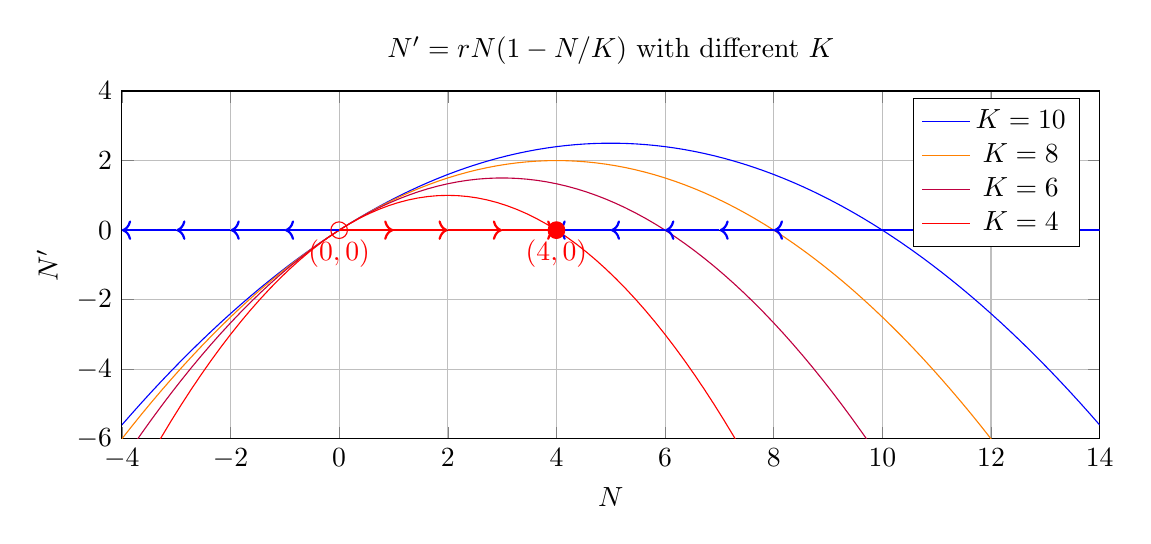
\begin{tikzpicture}
			\begin{axis}[
				title={\(N' = rN(1- N/K)\) with different \(K\)},
				xlabel={\(N\)},
				ylabel={\(N'\)},
				xmin=-4, xmax=14,
				ymin=-6, ymax=4,
				grid=major,
				width=14cm,
				height=6cm,
				]
			% the plot when r = 1 and K = 10
			\addplot[blue, domain=-4:14, samples=100]{x*(1-x/10)};
			% the plot when r = 1 and K = 8
			\addplot[orange, domain=-4:14, samples=100]{x*(1-x/8)};
			% the plot when r = 1 and K = 6
			\addplot[purple, domain=-4:14, samples=100]{x*(1-x/6)};
			% the plot when r = 1 and K = 4
			\addplot[red, domain=-4:14, samples=100]{x*(1-x/4)};

			% draw the x axis as black color
			\addplot[black, domain=-4:14, samples=100]{0};

			% add a hollow red point at (0,0) and add lebal to the red point 
			\addplot[only marks, mark=o, mark size=3pt, color=red] coordinates {(0,0)} node[anchor=north] {\((0,0)\)};
			% add a point at (4,0) and add lebal to the red point
			\addplot[only marks, mark=*, mark size=3pt, color=red] coordinates {(4,0)} node[anchor=north] {\((4,0)\)};

			% draw vector at (0, 0) toword (1,0) and change the size of the arrow
			\addplot[->, thick, color=red] coordinates {(0,0) (1,0)};
			% vector from (1,0) to (2,0)
			\addplot[->, thick, color=red] coordinates {(1,0) (2,0)};
			% vector from (2,0) to (3,0)
			\addplot[->, thick, color=red] coordinates {(2,0) (3,0)};
			% vector from (3,0) to (4,0)
			\addplot[->, thick, color=red] coordinates {(3,0) (4,0)};

			% vector from (-3,0) to (-4,0)
			\addplot[->, thick, color=blue] coordinates {(-3,0) (-4,0)};
			% vector from (-2,0) to (-3,0)
			\addplot[->, thick, color=blue] coordinates {(-2,0) (-3,0)};
			% vector from (-1,0) to (-2,0)
			\addplot[->, thick, color=blue] coordinates {(-1,0) (-2,0)};
			% vector from (0,0) to (-1,0)
			\addplot[->, thick, color=blue] coordinates {(0,0) (-1,0)};
			% vector from (5,0) to (4,0)
			\addplot[->, thick, color=blue] coordinates {(5,0) (4,0)};
			% vector from (6,0) to (5,0)
			\addplot[->, thick, color=blue] coordinates {(6,0) (5,0)};
			% vector from (7,0) to (6,0)
			\addplot[->, thick, color=blue] coordinates {(7,0) (6,0)};
			% vector from (8,0) to (7,0)
			\addplot[->, thick, color=blue] coordinates {(8,0) (7,0)};
			% vector from (14,0) to (8,0)
			\addplot[->, thick, color=blue] coordinates {(14,0) (8,0)};


			\legend{\(K = 10\), \(K = 8\), \(K = 6\), \(K = 4\)}
			\end{axis}
			\end{tikzpicture}

			I'm drawing vector field graph by using \(K=4\) as an example. No matter what \(K\) and \(r\) are, the range of vector will always be the same. The only difference is the scale of the graph. When \(K\) is larger, the graph will be more flat. When \(K\) is smaller, the graph will be more steep.
			
			The vector field graph with changing \(r\) is showing below:
			
			% the plot with different r
			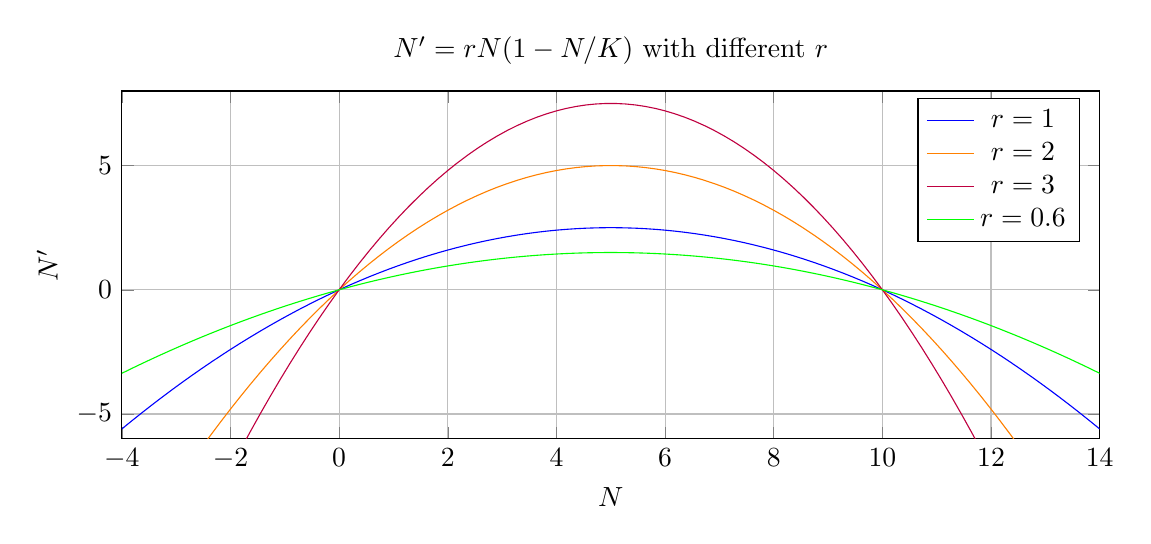
\begin{tikzpicture}
			\begin{axis}[
				title={\(N' = rN(1- N/K)\) with different \(r\)},
				xlabel={\(N\)},
				ylabel={\(N'\)},
				xmin=-4, xmax=14,
				ymin=-6, ymax=8,
				grid=major,
				width=14cm,
				height=6cm,
				]
			% the plot when r = 1 and K = 10
			\addplot[blue, domain=-4:14, samples=100]{x*(1-x/10)};
			% the plot when r = 2 and K = 10
			\addplot[orange, domain=-4:14, samples=100]{2*x*(1-x/10)};
			% the plot when r = 3 and K = 10
			\addplot[purple, domain=-4:14, samples=100]{3*x*(1-x/10)};
			% the plot when r = 0.6 and K = 10
			\addplot[green, domain=-4:14, samples=100]{0.6*x*(1-x/10)};
			
			\legend{\(r = 1\), \(r = 2\), \(r = 3\), \(r = 0.6\)}
			\end{axis}
			\end{tikzpicture}
			
			\item The largest growth rate is defined as \(N'/N\). Consider the model \(N' = rN(1- N/K)\), where \(r\) and \(K\) are positive constants. The largest growth rate is:
				\[\frac{N'}{N} = r(1- N/K)\]
				That indicated the largest growth rate is found when \(N\) is minimum. Since \(N\) is a positive number, the minimum value of \(N\) is \(0\). So the largest growth rate is \(r\).

			\item There are two fixed points in this model. One is \(N = 0\), the other one is \(N = K\). When \(N = 0\), \(N' = rN(1- N/K) = 0\). When \(N = K\), \(N' = rN(1- N/K) = 0\). So the fixed points are \((0,0)\) and \((K,0)\). By the vector field graph, we can see that \((0,0)\) is an unstable fixed point and \((K,0)\) is a stable fixed point.

			\item We will consider four inital condistions as: \(r =3,k=10\); \(r=1, k=10\); \(r=3, k=8\); \(r=1, k=8\). And we will take the constant $C=1$. The graph is showing below:

			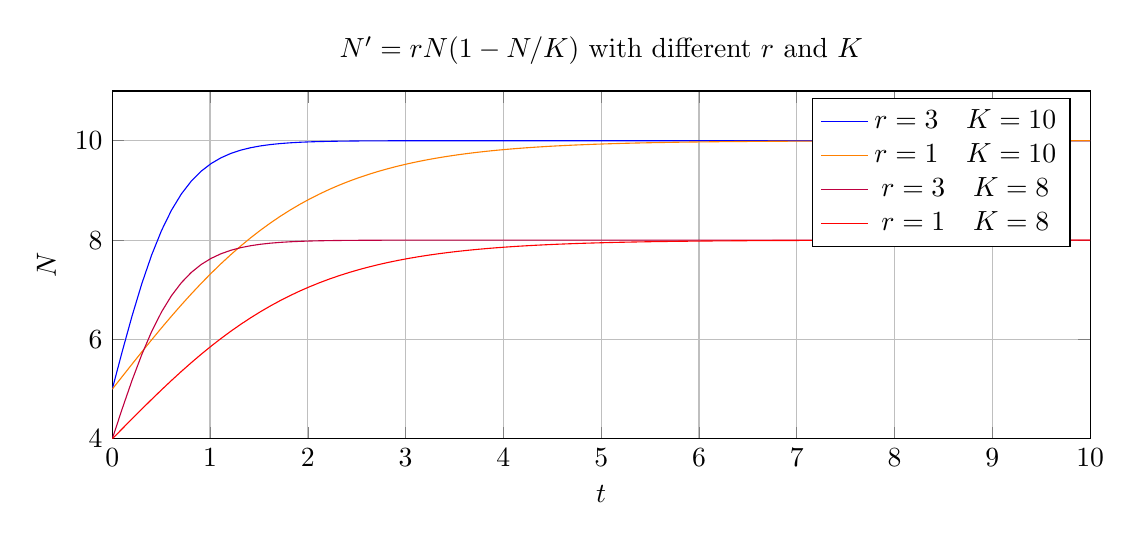
\begin{tikzpicture}
			\begin{axis}[
				title={\(N' = rN(1- N/K)\) with different \(r\) and \(K\)},
				xlabel={\(t\)},
				ylabel={\(N\)},
				xmin=0, xmax=10,
				ymin=4, ymax=11,
				grid=major,
				width=14cm,
				height=6cm,
				]
			% the plot when r = 3 and K = 10
			\addplot[blue, domain=0:10, samples=100]{10*e^(3*x)/(1+e^(3*x))};
			% the plot when r = 1 and K = 10
			\addplot[orange, domain=0:10, samples=100]{10*e^(x)/(1+e^(x))};
			% the plot when r = 3 and K = 8
			\addplot[purple, domain=0:10, samples=100]{8*e^(3*x)/(1+e^(3*x))};
			% the plot when r = 1 and K = 8
			\addplot[red, domain=0:10, samples=100]{8*e^(x)/(1+e^(x))};

			\legend{\(r = 3 \quad K=10\), \(r = 1 \quad K=10\), \(r = 3 \quad K=8\), \(r = 1 \quad K=8\)}
			\end{axis}
			\end{tikzpicture}
		\end{enumerate}
	
	\item Consider model \(N'=rN(1-N/K)(N/A-1)\) where $r>0$, $K>A>0$.
		\begin{enumerate}[i.]
			\item The vector field graph is showing below:

			% the plot with different K
			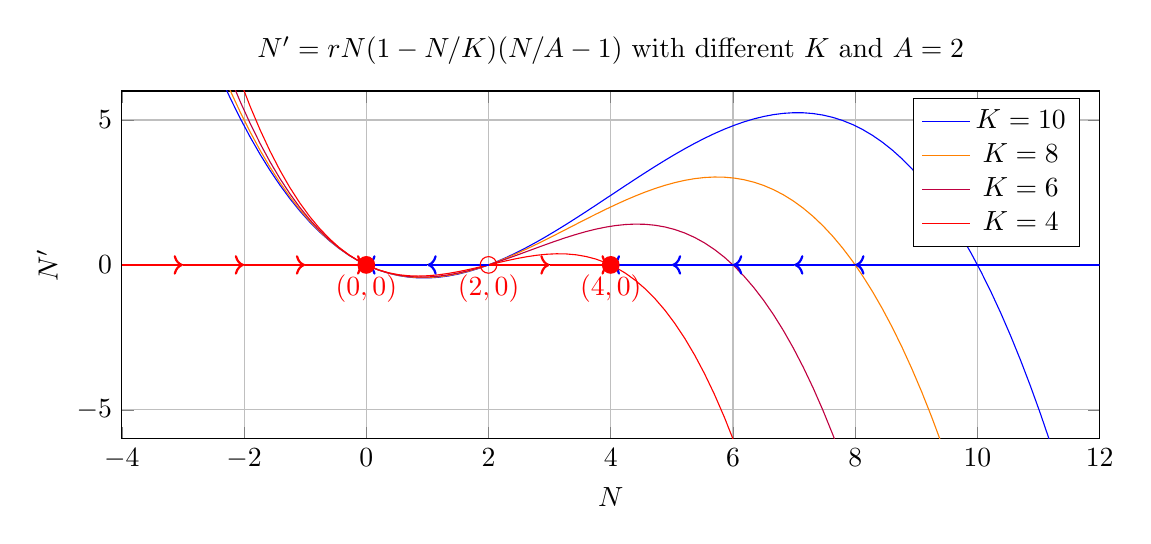
\begin{tikzpicture}
			\begin{axis}[
				title={\(N'=rN(1-N/K)(N/A-1)\) with different \(K\) and \(A=2\)},
				xlabel={\(N\)},
				ylabel={\(N'\)},
				xmin=-4, xmax=12,
				ymin=-6, ymax=6,
				grid=major,
				width=14cm,
				height=6cm,
				]
			% the plot when r = 1 and K = 10
			\addplot[blue, domain=-4:12, samples=100]{x*(1-x/10)*(x/2-1)};
			% the plot when r = 1 and K = 8
			\addplot[orange, domain=-4:12, samples=100]{x*(1-x/8)*(x/2-1)};
			% the plot when r = 1 and K = 6
			\addplot[purple, domain=-4:12, samples=100]{x*(1-x/6)*(x/2-1)};
			% the plot when r = 1 and K = 4
			\addplot[red, domain=-4:12, samples=100]{x*(1-x/4)*(x/2-1)};

			% draw the x axis as black color
			\addplot[black, domain=-4:12, samples=100]{0};
			
			% add a red point at (0,0) and add lebal to the red point
			\addplot[only marks, mark=*, mark size=3pt, color=red] coordinates {(0,0)} node[anchor=north] {\((0,0)\)};
			% add a hollow red point at (2,0) and add lebal to the red point
			\addplot[only marks, mark=o, mark size=3pt, color=red] coordinates {(2,0)} node[anchor=north] {\((2,0)\)};
			% add a red point at (4,0) and add lebal to the red point
			\addplot[only marks, mark=*, mark size=3pt, color=red] coordinates {(4,0)} node[anchor=north] {\((4,0)\)};

			% draw vector at (1, 0) toword (0,0) and change the size of the arrow
			\addplot[->, thick, color=blue] coordinates {(1,0) (0,0)};
			% vector from (2,0) to (1,0)
			\addplot[->, thick, color=blue] coordinates {(2,0) (1,0)};
			% vector from (5,0) to (4,0)
			\addplot[->, thick, color=blue] coordinates {(5,0) (4,0)};
			% vector from (6,0) to (5,0)
			\addplot[->, thick, color=blue] coordinates {(6,0) (5,0)};
			% vector from (7,0) to (6,0)
			\addplot[->, thick, color=blue] coordinates {(7,0) (6,0)};
			% vector from (8,0) to (7,0)
			\addplot[->, thick, color=blue] coordinates {(8,0) (7,0)};
			% vector from (12,0) to (8,0)
			\addplot[->, thick, color=blue] coordinates {(12,0) (8,0)};

			% vector from (-4,0) to (-3,0)
			\addplot[->, thick, color=red] coordinates {(-4,0) (-3,0)};
			% vector from (-3,0) to (-2,0)
			\addplot[->, thick, color=red] coordinates {(-3,0) (-2,0)};
			% vector from (-2,0) to (-1,0)
			\addplot[->, thick, color=red] coordinates {(-2,0) (-1,0)};
			% vector from (-1,0) to (0,0)
			\addplot[->, thick, color=red] coordinates {(-1,0) (0,0)};
			% vector from (2,0) to (3,0)
			\addplot[->, thick, color=red] coordinates {(2,0) (3,0)};
			% vector from (3,0) to (4,0)
			\addplot[->, thick, color=red] coordinates {(3,0) (4,0)};

			\legend{\(K = 10\), \(K = 8\), \(K = 6\), \(K = 4\)}
			\end{axis}
			\end{tikzpicture}
			
			\item The largest growth rate is defined as \(N'/N\). Consider the model \(N'=rN(1-N/K)(N/A-1)\), where \(r>0\), \(K>A>0\). The largest growth rate is:
				\[\frac{N'}{N} = r(1-N/K)(N/A-1)\]
				By setting $\frac{N'}{N}' = 0$, we can find the largest growth rate is when $N = (A+K)/2$. So the largest growth rate is: $r(1-(A+K)/2K)((A+K)/2A-1)$.

			\item There are three fixed points in this model. One is \(N = 0\), the other one is \(N = K\), the last one is \(N = A\). When \(N = 0\), \(N' = rN(1-N/K)(N/A-1) = 0\). When \(N = K\), \(N' = rN(1-N/K)(N/A-1) = 0\). When \(N = A\), \(N' = rN(1-N/K)(N/A-1) = 0\). So the fixed points are \((0,0)\), \((K,0)\) and \((A,0)\). By the vector field graph, we can see that \((0,0)\) is a stable fixed point, \((K,0)\) is a stable fixed point and \((A,0)\) is an unstable point.

			\item There is the plot showing below:

				\begin{tikzpicture}
					\begin{axis}[
						title={\(N'=rN(1-N/K)(N/A-1)\) with \(r=3\) and \(K=10, A=2\)},
						xlabel={$t$}, 
						ylabel={$x(t)$},
						grid=major,
						width=14cm,
						height=14cm,
						]
						\addplot[quiver={u=\thisrow{U},v=\thisrow{V},scale arrows=0.2},-stealth, color=blue] table [x=T, y=X, col sep=comma] {vector_field_data.csv};
					\end{axis}
				\end{tikzpicture}

			This is plot is using Python to generate. The code is here. The export data is in the file \texttt{vector\_field\_data.csv}.

		\end{enumerate}

	\item The model in (b) incorporate the threshold. The point $0$ is a stable equilibrium point. But the point $A$ is an unstable equilibrium point. The point $K$ is a stable equilibrium point which is a carrying capcity point. But the point $K$ is not stable point like a threshold, which is not model (a) have. The model in (b) is more realistic than the model in (a).

	
\end{enumerate}















\end{document}

